%%%% ijcai26.tex

\typeout{IJCAI--ECAI 26 Instructions for Authors}

% These are the instructions for authors for IJCAI--ECAI 26.

\documentclass{article}
%\pdfpagewidth=8.5in
%\pdfpageheight=11in

% The file ijcai26.sty is a copy from ijcai22.sty
% The file ijcai22.sty is NOT the same as previous years'
\usepackage{ijcai26}

% Use the postscript times font!
\usepackage{times}
\usepackage{soul}
\usepackage{url}
\usepackage[hidelinks]{hyperref}
\usepackage[T2A]{fontenc}
\usepackage[utf8]{inputenc}
\usepackage[english,russian]{babel}
\usepackage{tempora}
\usepackage[small]{caption}
\usepackage{graphicx}
\usepackage{amsmath}
\usepackage{amsthm}
\usepackage{booktabs}
\usepackage{algorithm}
\usepackage{algorithmic}
\usepackage[switch]{lineno}

% Comment out this line in the camera-ready submission
% \linenumbers

\urlstyle{same}

% the following package is optional:
%\usepackage{latexsym}

% See https://www.overleaf.com/learn/latex/theorems_and_proofs
% for a nice explanation of how to define new theorems, but keep
% in mind that the amsthm package is already included in this
% template and that you must *not* alter the styling.
% \newtheorem{example}{Example}
% \newtheorem{theorem}{Theorem}

% Following comment is from ijcai97-submit.tex:
% The preparation of these files was supported by Schlumberger Palo Alto
% Research, AT\&T Bell Laboratories, and Morgan Kaufmann Publishers.
% Shirley Jowell, of Morgan Kaufmann Publishers, and Peter F.
% Patel-Schneider, of AT\&T Bell Laboratories collaborated on their
% preparation.

% These instructions can be modified and used in other conferences as long
% as credit to the authors and supporting agencies is retained, this notice
% is not changed, and further modification or reuse is not restricted.
% Neither Shirley Jowell nor Peter F. Patel-Schneider can be listed as
% contacts for providing assistance without their prior permission.

% To use for other conferences, change references to files and the
% conference appropriate and use other authors, contacts, publishers, and
% organizations.
% Also change the deadline and address for returning papers and the length and
% page charge instructions.
% Put where the files are available in the appropriate places.


% PDF Info Is REQUIRED.

% Please leave this \pdfinfo block untouched both for the submission and
% Camera Ready Copy. Do not include Title and Author information in the pdfinfo section
%\pdfinfo{
%/TemplateVersion (IJCAI.2026.0)
%}

\title{SparseDR: Дифференцируемый рендеринг разреженных функций расстояния}

% Single author syntax
% \author{
%     Author Name
%     \affiliations
%     Affiliation
%     \emails
%     email@example.com
% }

% Multiple author syntax (remove the single-author syntax above and the \iffalse ... \fi here)
% \iffalse
\author{
Алексей Будак$^{1}$
\and
Альберт Гарифуллин$^1$\and
Владимир Фролов$^{2}$
\affiliations
$^1$МГУ имени М.В. Ломоносова\\
$^2$Институт Искусственного Интеллекта, МГУ имени М.В. Ломоносова\\
\emails % usually included
\{ alexey.budak, albert.garifullin, vladimir.frolov \}@graphics.cs.msu.ru
}
% \fi

\begin{document}

\maketitle

\begin{abstract}
	Мы представляем SparseDR -- новый алгоритм дифференцируемого рендеринга, разработанный для разрежённых представлений на основе функций расстояния со знаком (signed distance functions, SDF). Мы используем представление Sparse Brick Set и предлагаем адаптацию процедуры редистансинга для разреженных SDF. Это позволяет SparseDR превосходить существующие методы по точности восстановления поверхности за счёт увеличения эффективного разрешения SDF представления. SparseDR эффективно реализован на C++ и Vulkan, достигая в несколько раз меньшего времени реконструкции по сравнению с другими методами.
\end{abstract}

\section{Введение}

Функция расстояния со знаком (SDF) -- это непрерывное неявное представление геометрии, хранящее кратчайшее евклидово расстояние от любой точки пространства до ближайшей поверхности, при этом знак указывает на внутренние и внешние области. Она зарекомендовала себя как представление поверхности объекта, удобное для дифференцируемого рендеринга, обеспечивая устойчивую и относительно простую градиентную оптимизацию \cite{DRSDF24}.
  
  В дифференцируемом рендеринге на основе SDF каждый шаг градиентного спуска обновляет значения расстояния в ячейках сетки, вследствие чего сетка перестаёт строго удовлетворять свойству SDF. Для решения этой проблемы существующие методы обычно применяют процесс \textit{редистансинга} -- процедуру, при которой значения в сетке пересчитываются так, чтобы каждая ячейка хранила корректное расстояние до поверхности \cite{DETRIXHE201346}. Это делает дифференцируемый рендеринг на основе SDF на разреженных структурах данных нетривиальной задачей, поэтому все существующие методы опираются на регулярные сетки. К сожалению, такой подход приводит к высоким затратам памяти и требует большой объём вычислений, при этом точность реконструкции остаётся ограниченной максимальным разрешением сетки. В нашей работе предлагается решение этой проблемы, смягчающее указанные ограничения за счёт более эффективных структур данных и методов выборки:
  
  \begin{itemize}
    \item Мы предлагаем адаптацию дифференцируемого рендеринга SDF под разреженную структуру данных, что увеличивает эффективное разрешение представления SDF и тем самым повышает точность восстановления поверхности.
    \item Мы адаптируем редистансинг к разреженным структурам данных, разделяя её на два отдельных алгоритма: локальный и глобальный редистансинг. 
  \end{itemize}

    \begin{figure}[t]
    	\centering
    	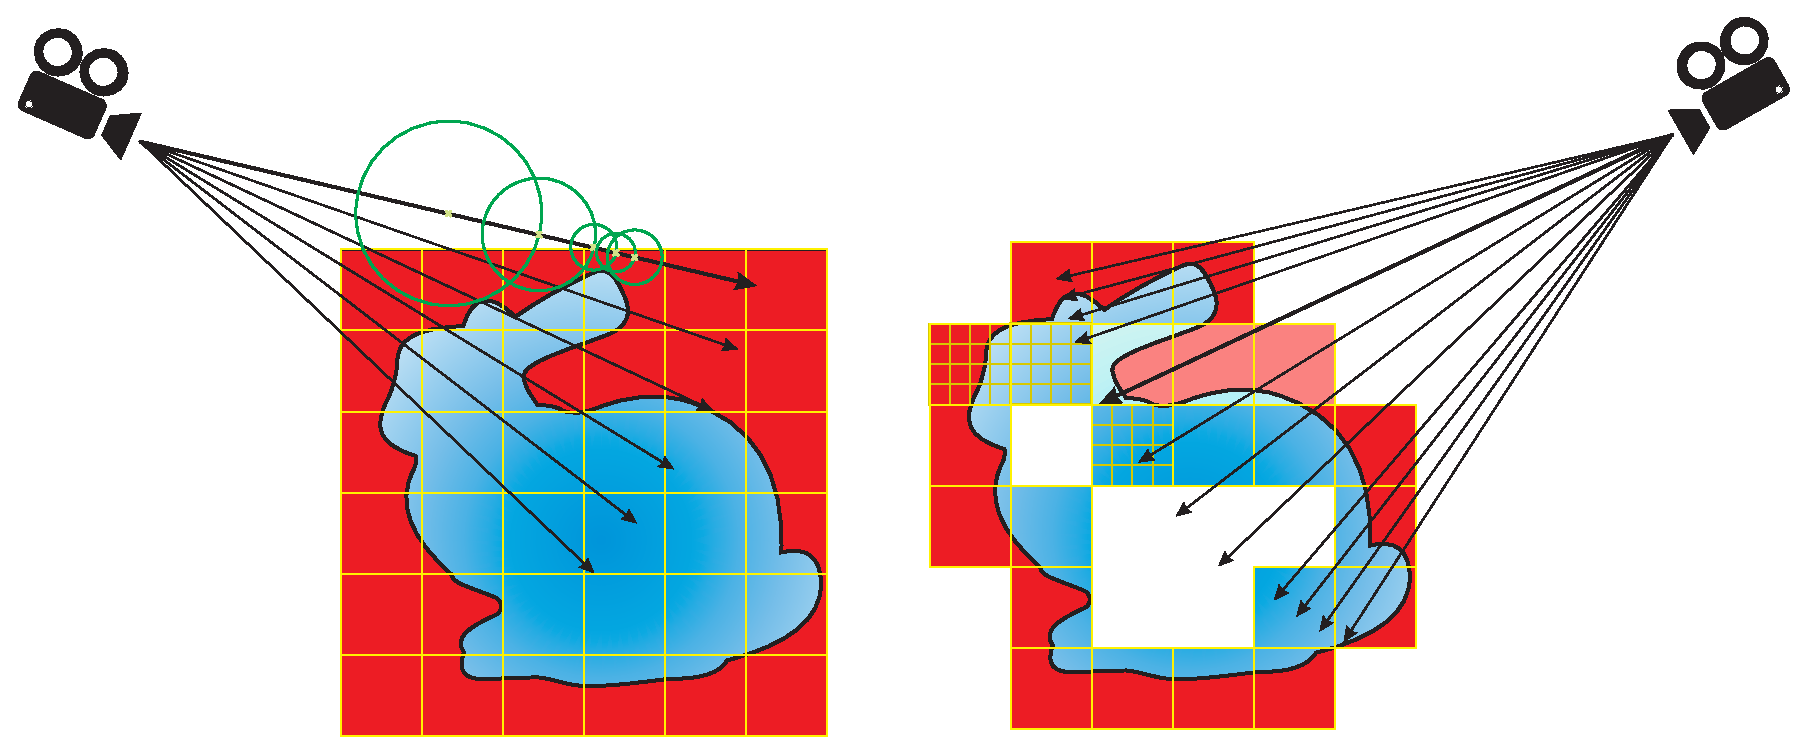
\includegraphics[width=\columnwidth,keepaspectratio]{figures/header.eps}
    	\caption{Существующие методы (слева) используют плотную SDF сетку для представления поверхности, sphere tracing для пересечения луча со сценой и равномерное семплирование изображения при генерации лучей. SparseDR (справа) использует Sparse Brick Set, где луч пересекает каждый брик на своём пути, пока не достигнет поверхности. Также применяется адаптивное семплирование для граничного интеграла, пускающее больше лучей в области релаксированной границы. Красный и синий цвета соответствуют положительным и отрицательным значениям SDF соответственно.}
    	\label{fig:header}
    \end{figure}

\section{Связанные работы}

Представление SDF на регулярной сетке в существующих работах \cite{DRSDF22,DRSDF24,ManyWorld25} имеет три основных ограничения: (1) значительное потребление памяти, особенно при использовании фреймворков автоматического дифференцирования, таких как DrJit \cite{drjit} или PyTorch \cite{pytorch}; (2) медленное вычисление пересечения луча с поверхностью на основе sphere tracing; (3) дорогостоящий алгоритм редистансинга, который распространяет изменённые значения SDF по всей сетке. В нашей работе показано, как эти компоненты -- структура данных, пересечение лучей и редистансинг -- могут быть эффективно объединены.
   

\section{Предложенный метод}

SparseDR использует в качестве представления Sparse Brick Set (SBS) \cite{soderlund2022ray}, представляющий собой гибрид иерархического и регулярного представлений (Рис. \ref{fig:header}). Вся сцена кодируется в виде иерархии ограничивающих объёмов (BVH); её листья хранят небольшие регулярные SDF сетки, например 4×4×4 вокселя, называемые бриками. Для вычисления градиентов мы адаптируем метод релаксированной границы из \cite{DRSDF24}, который используем в качестве базового.

Предлагаемый процесс оптимизации состоит из нескольких эпох, каждая из которых включает несколько шагов градиентного спуска. В начале функция расстояния инициализируется сферой, заданной на сетке низкого разрешения (например, $32^3$). На каждой итерации оцениваются градиенты и обновляются значения функции расстояния с использованием шага градиентного спуска, за которым следуют регуляризация и локальный редистансинг (см. Рис. \ref{fig:redist}). В конце эпохи выполняются два шага: апсемплинг и глобальный редистансинг. После последней эпохи выполняется только глобальный редистансинг.

\textbf{Оценка градиентов.} Ключевой особенностью SparseDR является переход от регулярной сетки к Sparse Brick Set. Для SBS строится дерево BVH, где каждый листовой узел хранит один брик. Вместо sphere tracing мы используем более быстрый метод Ньютона для пересечения луча с SDF \cite{soderlund2022ray}. Луч сначала обходит BVH; если обнаруживается пересечение с листовым узлом, далее выполняется пересечение с вокселями внутри брика. Луч проходит через каждый лист BVH на своём пути, пока не достигнет поверхности или пока на его пути не останется листьев. Метод Ньютона был модифицирован для поиска точек релаксированной границы: внутри вокселя потенциальная точка релаксированной границы находится как корень квадратного уравнения, после чего проверяется, что значение SDF в этой точке ниже порогового. Случай, когда локальный минимум находится на границе вокселя, обрабатывается отдельно.

SparseDR реализован на C++ и Vulkan и не использует автоматическое дифференцирование, то есть все производные были получены аналитически. В шейдере мы накапливаем цвет пикселя группами по 16 семплов, сохраняя информацию о вокселях, с которыми пересеклись эти лучи, в массиве фиксированного размера. Каждые 16 семплов, либо после последнего, градиенты накапливаются с использованием атомарных операций.

SparseDR опционально использует дополнительный проход, в котором семплируются только пиксели, содержащие границы, и вычисляется только граничный интеграл, что устраняет необходимость вычисления цвета. Это позволяет удешевить обработку граничных семплов и снижает дисперсию.

\begin{figure}
    \centering
    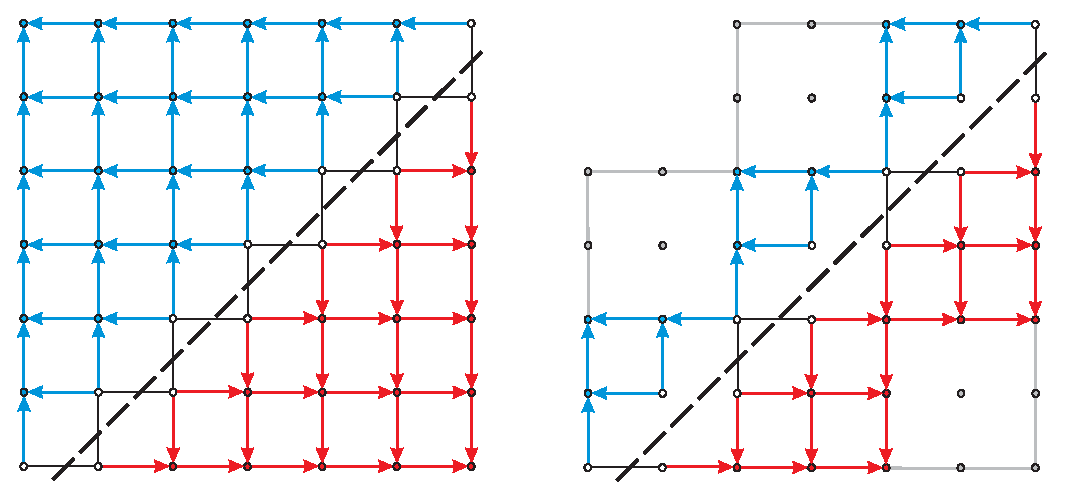
\includegraphics[width=\columnwidth,keepaspectratio]{figures/redistancing.eps}
    \caption{Сравнение глобального алгоритма редистансинга на плотной сетке (слева) с локальным редистансингом (справа) для SBS; брики имеют размер 3×3 дистанции. Точки представляют значения расстояния. Красные и синие точки соответствуют расстояниям вне и внутри объекта соответственно. Пунктирная линия обозначает поверхность, заданную значениями расстояния, окрашенными в белый цвет. Стрелки показывают порядок обновления значений. Локальный редистансинг игнорирует брики без поверхности (серые).}

    \label{fig:redist}
\end{figure}

\textbf{Локальный редистансинг.}
Мы реализовали две версии редистансинга: локальную и глобальную (Рис. \ref{fig:redist}). В предлагаемом методе расстояния в бриках без поверхности не обязаны строго удовлетворять свойству SDF в процессе оптимизации. Поэтому на каждой итерации применяется локальная версия, в которой расстояния пересчитываются только внутри бриков, содержащих поверхность. На практике локального редистансинга достаточно, поскольку наш метод пересечения луча с поверхностью опирается исключительно на значения расстояний внутри пересекаемых брирков. Однако такой подход может приводить к несогласованности расстояний между соседними бриками, поэтому в конце каждой эпохи мы выполняем глобальный редистансинг.


\begin{figure}[t]
    \centering
    
\includegraphics[width=0.7\columnwidth,keepaspectratio]{figures/collage_sparsedr_new.pdf}
    \caption{ Примеры реконструкции для разных эпох. }
    \label{fig:collage}
\end{figure}

\textbf{Апсемплинг и глобальный редистансинг.} Глобальный редистансинг обновляет значения расстояний через пустые области между бриками, экстраполируя значения между их гранями. Для каждой грани, не имеющей непосредственного соседа, находятся ближайшие соседние брики, после чего одна из их граней выбирается в качестве источника экстраполяции. Поиск соседей выполняется один раз, после чего экстраполяция производится после каждой итерации fast-sweeping алгоритма. На каждом шаге сохраняется значение с меньшим модулем расстояния между экстраполированным и существующим значением. Процесс перерасчёта завершается шагом fast-sweeping алгоритма, который распространяет экстраполированные расстояния по всей области.

На этапе повышения разрешения сначала выполняется разрежение SBS. На этом этапе сохраняются только брики, содержащие поверхность, а также все соседние брики в радиусе одного брика (включая диагональных соседей). Если какие-либо из соседних бриков отсутствуют, они добавляются на данном этапе. Этот шаг необходим, поскольку области, соответствующие поверхности, в противном случае могут не иметь соответствующего покрытия бриками. Таким образом, данная процедура не только уменьшает общий размер модели, но и устраняет потенциальное ограничение по сравнению с базовым методом. Следом за разрежением разрешение каждого брика удваивается, после чего он разбивается на восемь меньших бриков исходного размера. Новые значения дистанций вычисляются с использованием трилинейной интерполяции. После повышения разрешения выполняется шаг глобального редистансинга, на котором пересчитываются все дистанции, обеспечивая корректность полученного SDF представления.

\section{Эксперименты}

Эксперименты с базовым методом проводились с использованием исходной конфигурации, приведённой в официальной реализации \cite{DRSDF24Repo}. Единственными изменениями являются количество ракурсов, размер батча и размеры эпох. Для обеспечения согласованности между экспериментами использовалась одинаковая схема освещения: два направленных источника света с направлениями (1,1,1) и (-1,-1,-1), а также фоновое освещение. Эксперименты проводились на шести моделях. Четыре модели взяты из репозитория 3D-сканирования Стэнфорда: Armadillo, Asian Dragon, Stanford Bunny и Happy Buddha. Две другие модели -- это скан Нефертити \cite{nefertitihack} и Utah Teapot. Реконструкция выполнялась с использованием 16 ракурсов, равномерно распределённых по сфере вокруг сцены и сгенерированных алгоритмом из \cite{DRSDF24Repo}. Размер батча составляет 4 ракурса; разрешение изображений -- 1024×1024.

Полный процесс оптимизации состоял из 1000 шагов, апсемплинг применялся на шагах 200, 400, 600, 700, 800, и 900. Аппаратная конфигурация: AMD Ryzen 9 7950X CPU и NVIDIA GeForce RTX 4090 GPU. Некоторые примеры реконструкции приведены на Рис. \ref{fig:collage}.

\begin{figure}[t]
    \centering
    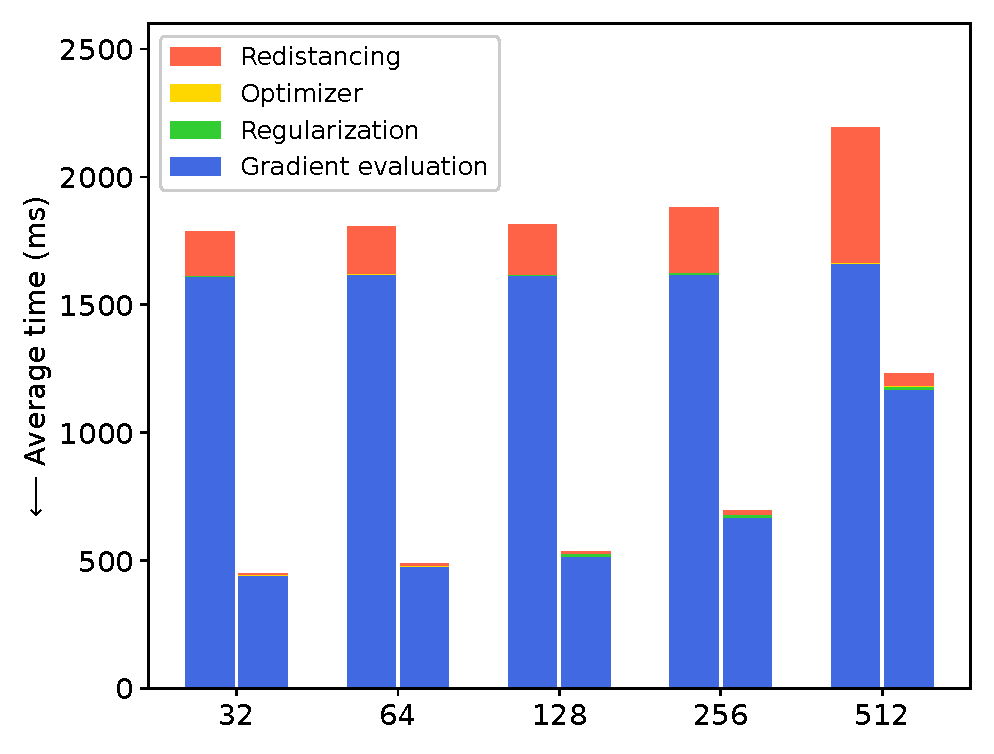
\includegraphics[width=\columnwidth,keepaspectratio]{figures/time_1iter.eps}
    \caption{ Среднее время выполнения одной итерации. Для каждого размера сетки слева показано время базового метода, справа -- SparseDR с соответствующим разрешением. }
    \label{fig:iter_time}
\end{figure}

\begin{figure}[t]
    \centering
    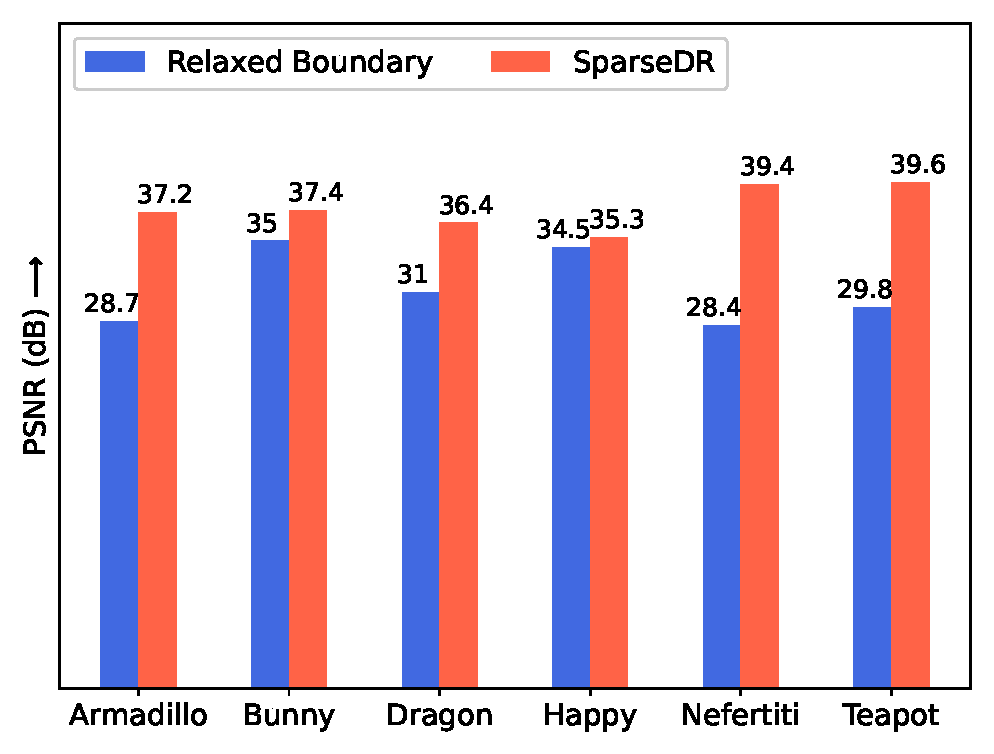
\includegraphics[width=\columnwidth,keepaspectratio]{figures/psnr_comp.eps}
    \caption{ Среднее по ракурсам значение PSNR для моделей. }
    \label{fig:comp_psnr}
\end{figure}

Рис. \ref{fig:iter_time} показывает среднее время реконструкции по всем моделям на эпоху для SparseDR и базового метода; эпохи помечены размером SDF-сетки соответствующего разрешения. Под «оценкой градиента» понимается последовательный рендеринг со всех ракурсов из текущего батча. Рис. \ref{fig:comp_psnr} представляет среднее качество реконструкции по всем точкам обзора для SparseDR и базового метода. Таблица \ref{tab:comp_size} иллюстрирует размеры моделей для эпох. Для базового метода приводится только размер сетки; для SparseDR указываются как размер SBS, так и его BVH. Результаты демонстрируют увеличение скорости и качества реконструкции по сравнению с базовым методом, при этом рост размера SBS на порядок меньше, чем у SDF-сетки.


\begin{table}
    \centering
    \begin{tabular}{cccccc} % 1, 2, 4, 5, 7,
        \toprule
        Представление & $64^3$ & $128^3$ & $512^3$ & $1024^3$ & $2048^3$  \\
        \midrule[\heavyrulewidth]
        Базовый      & \textbf{1} & \textbf{8} & 512  & 4096* & 32768* \\
        Наш(Armadillo) &   3.1 & 14.1 & \textbf{126.2} & \textbf{514.2} & \textbf{1074.2}  \\
        \cmidrule(lr){1-1}  \cmidrule(lr){2-6}
        Базовый      & \textbf{1} & \textbf{8} & 512  & 4096* & 32768* \\
        Наш(Bunny) &   2.9 & 11.4 & \textbf{195.1} & \textbf{775.3} & \textbf{3093.8}  \\
        \cmidrule(lr){1-1}  \cmidrule(lr){2-6}
        Базовый      & \textbf{1} & 8   & 512  & 4096* & 32768* \\
        Наш(Dragon) &   1.8 & \textbf{4.8} & \textbf{67.9} & \textbf{275.6} & \textbf{1154.6}  \\
        \cmidrule(lr){1-1}  \cmidrule(lr){2-6}
        Базовый      & \textbf{1} & 8   & 512  & 4096* & 32768* \\
        Наш(Happy) &   1.5 & \textbf{4.9} & \textbf{88.5} & \textbf{373.9} & \textbf{1562.8}  \\
        \cmidrule(lr){1-1}  \cmidrule(lr){2-6}
        Базовый      & \textbf{1} & 8   & 512  & 4096* & 32768* \\
        Наш(Nefertiti) &   2.2 & \textbf{7.3} & \textbf{114.1} & \textbf{459.0} & \textbf{1845.3}  \\
        \cmidrule(lr){1-1}  \cmidrule(lr){2-6}
        Базовый      & \textbf{1} & 8   & 512  & 4096* & 32768* \\
        Наш(Teapot) & 1.7 & \textbf{6.3} & \textbf{96.4} & \textbf{392.1} & \textbf{1597.7}  \\
        \bottomrule
    \end{tabular}
    \caption{Размеры моделей для метода релаксированной границы и SparseDR. Все величины указаны в МБ. Звёздочкой обозначены теоретические значения, так как мы не смогли получить их в нашей аппаратной конфигурации (OOM в Dr.JIT).}
    \label{tab:comp_size}
\end{table}

\section{Заключение}

В данной работе мы представляем SparseDR -- метод дифференцируемого рендеринга на основе разреженного SDF представления. Развивая подход \cite{DRSDF24}, мы используем преимущества Sparse Brick Sets, чтобы превзойти базовый метод при одновременном снижении потребления памяти на порядок. В будущих работах планируется сосредоточиться на повышении производительности. Мы полагаем, что предложенный подход обладает потенциалом для дальнейшего повышения эффективности, в частности за счёт более точной оценки градиентов и уменьшения количества семплов на пиксель.


\section*{Этическое заявление}

Этические проблемы отсутствуют.

\section*{Благодарности}

Алексей Будак и Альберт Гарифуллин работали с поддержкой Министерства Экономического Развития Российской Федерации в соответствии с соглашением о субсидировании (соглашение 000000C313925P4H0002; грант № 139-15-2025-012).

%% The file named.bst is a bibliography style file for BibTeX 0.99c
\bibliographystyle{named}
\bibliography{sparsedr}

\end{document}

